\ifx\ucebnice\undefined
\documentclass[a4paper,10pt,oneside]{article}
\usepackage{latexsym}
\usepackage{amsmath}
\usepackage{amsfonts}
\usepackage{amsthm}
\usepackage{amssymb}
\usepackage{fncylab}
\usepackage{comment}
\usepackage{float}
\usepackage{wrapfig}
\usepackage{tikz}
\usepackage{tikz-qtree}
\usepackage{url}
\usepackage[bookmarks, colorlinks=false, 
            pdftitle={Úvod do programování --- Algoritmy},
            pdfauthor={Jonathan L. Verner}, 
            pdfsubject={Algoritmy a složitost}, 
            pdfkeywords={algoritmus, složitost, Python, třídění, grafy},
            bookmarksdepth=3
            ]{hyperref}
\usepackage[margin=1cm]{geometry}
\usetikzlibrary{decorations.fractals,chains,fit,shapes,patterns}
\usepackage[utf8]{inputenc}
\usepackage[T1]{fontenc}
\usepackage{attachfile}
\relpenalty=9999
\binoppenalty=9999


%----------definitions---------------------------


%math definitions

\newcommand{\R}{\mathbb R}
\newcommand{\C}{{\mathcal C}}
\newcommand{\F}{{{\mathcal F}}}
\newcommand{\U}{{{\mathcal U}}}
\newcommand{\V}{{{\mathcal V}}}
\newcommand{\cont}{{\mathfrak{c}}}
\newcommand{\force}{\Vdash}
\newcommand{\pw}{{{\mathcal P}}}
\newcommand{\MU}{{\mathbb{M}_{\mathcal{U}}}}
\newcommand{\pomega}{\pw(\omega)}


\newcommand{\src}[3]{%
\begin{program}%
\caption{#2\hfill%
\attachfile[author={Jonathan Verner},
            description={Source code for #2},
            mimetype={text/x-python},
            print=false,
            icon={Paperclip}]{kod/#1}}
\label{#3}\includecode[Python]{kod/#1}
\end{program}}


%---------numbering of the theorems------------
 \swapnumbers

 \newtheorem*{theorem*}{Theorem}
 \newtheorem{theorem}[subsection]{Theorem}
 \newtheorem{proposition}[subsection]{Proposition}
 \newtheorem{observation}[subsection]{Observation}
 \newtheorem{fact}[subsection]{Fact}
 \newtheorem{lemma}[subsection]{Lemma}
 \theoremstyle{definition}
 \newtheorem{definition}[subsection]{Definice}
 \newtheorem{question}[subsection]{Problém}
 \newtheorem{ukol}{Úloha}
 \newtheorem{cviceni}[subsection]{Cvičení}
 \newtheorem{cviceniH}[subsection]{Cvičení (*)}
 \newtheorem*{reseniIMPL*}{Řešení}
 \specialcomment{reseni}{\begin{reseniIMPL*}}{\end{reseniIMPL*}}
 \excludecomment{reseni}
 \excludecomment{todo}
 \newtheorem*{comments*}{Komentáře}
 \newtheorem*{definition*}{Definice}
 \newtheorem*{question*}{Question}
 \newtheorem{notation}[subsection]{Notation}
 \newtheorem{remark}[subsection]{Poznámka}
 \newtheorem{remark*}[subsection]{Poznámka}
 \newtheorem*{note}{Poznámka}
 \newtheorem*{ack}{Acknowledgements}
 \floatstyle{ruled}
 \newfloat{program}{htbp}{listings}[section]
 \floatname{program}{Algoritmus}
 
 \hypersetup{
    colorlinks,%
    citecolor=black,%
    filecolor=black,%
    linkcolor=black,%
    urlcolor=black
}
 
\pdfinfo{
      /Author (Jonathan Verner)
      /Title (ALG110006 Úvod do programování: Poznámky k přednášce, LS)
      /Subject (programování, algoritmy)
      /Keywords (quicksort,heapsort,dijsktra,graph,euclid)
   }
\include{pythonlisting}

\lstset{
numbers=left,
stepnumber=1,
numbersep=5pt,
numberstyle=\small\color{black}
}
%-------------opening--------------------------
\begin{document}
\title{}

% \author{Jonathan Verner}
% \address{Department of Logic, Charles University\\
% Palachovo nám. 2\\ 116 38 Praha 1, Czech Republic}
% \email{jonathan.verner{@}ff.cuni.cz}
%\thanks{The author was partially supported by }

%\subjclass[2010]{Primary }
%\keywords{}

%\begin{abstract}
%\end{abstract}
%\maketitle
\thispagestyle{empty}
\pagestyle{empty}
%\hsize=16cm
\parindent=0cm
\parskip=0.2cm

\setcounter{section}{4}
\fi
\section{Grafové algoritmy}

Matematický pojem grafu formalizuje situaci, kdy máme danou nějakou množinu vrcholů (v reálném světě například množinu měst), které
jsou pospojovány hranami (v reálném světě například silinice). Příkladem takového grafu je následující obrázek:

\begin{center}
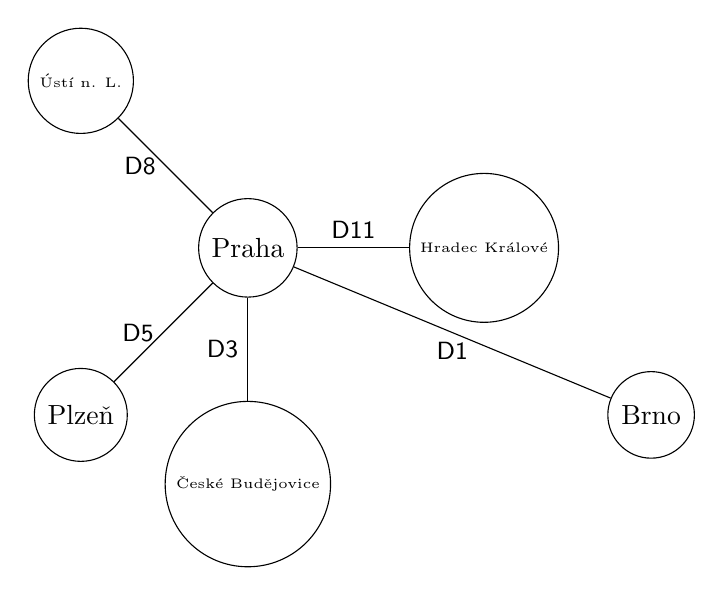
\begin{tikzpicture}[node distance=3cm]
\tikzstyle{vertex}=[draw,circle]
\node [vertex] (a){Praha};
\node [vertex,right of=a] (b){{\tiny Hradec Králové}};
\node [vertex,below right of=b] (c){Brno};
\node [vertex,below left of=a] (d){Plzeň};
\node [vertex,below of=a] (e){{\tiny České Budějovice}};
\node [vertex,above left of=a] (f){{\tiny Ústí n. L.}};
\path[every node/.style={font=\sffamily\small}]
    (a) edge node [above] {D11} (b)
    (a) edge node [below] {D1} (c)
    (a) edge node [left] {D5} (d)
    (a) edge node [left] {D3} (e)
    (a) edge node [left] {D8} (f);
\end{tikzpicture}
\end{center}

Formální definice grafu (a některých dalších pojmů) následuje:

\begin{definition} \emph{Neorientovaný graf} je dvojice množin $(V,E)$, kde $V$ je množina vrcholů a $E\subseteq V\times V$ je symetrická (t.j. $vEw\rightarrow wEv$),
irreflexivní relace (t.j. $\neg vEw$), udávající hrany (E z anglického edge). Není-li relace symetrická, mluvíme o \emph{orientovaném grafu}. Není-li relace
irreflexivní, v grafu uvažujeme i tzv. smyčky --- hrany vedoucí z vrcholu $v$ opět do vrcholu~$v$. \emph{Stupněm vrcholu} $v\in V$ rozumíme velikost množiny
$\{w\in V:vEw\}$ a značíme ho $deg(v)$ --- t.j. je to počet vrcholů, do nichž vede z $v$ hrana.
\end{definition}

Těmito objekty se zabývá (rozsáhlá a zajímavá) matematická teorie grafů. Jedním z problémů, který se dá v řeči grafů formulovat
je následující otázka:

\begin{question}\label{question:barvenimapy} Mějme dánu mapu regionů nějakého státu. Je vždy možné obarvit každý region jednou ze čtyř barev tak, aby žádné dva sousední
regiony neměly stejnou barvu?
\end{question}

Zkusme tuto otázku formulovat v řeči grafů. Máme-li dánu mapu, vytvoříme z ní graf tak,
že každému regionu bude odpovídat vrchol grafu a vrcholy sousedících regionů budou
spojeny hranou. Můžeme tedy zkusit formulovat otázku \ref{question:barvenimapy}
následujícím způsobem:

\begin{question}\label{question:generalcoloring} Lze vrcholy každého grafu obarvit čtyřmi barvami tak, aby sousední 
vrcholy měly vždy různou barvu?
\end{question}

Takto formulovaná otázka má však velmi jednoduchou odpověď. Uvažujme následující graf:

\begin{center}
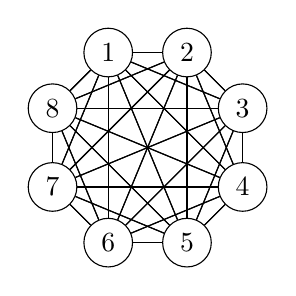
\begin{tikzpicture}[node distance=1cm]
\tikzstyle{vertex}=[draw,circle]
\node [vertex] (a){1};
\node [vertex,right of=a] (b){2};
\node [vertex,below right of=b] (c){3};
\node [vertex,below of=c] (d){4};
\node [vertex,below left of=d] (e){5};
\node [vertex,left of=e] (f){6};
\node [vertex,above left of=f] (g){7};
\node [vertex,above of=g] (h){8};
\path[every node/.style={font=\sffamily\small}]
    (a) edge node [above] {} (b)
    (a) edge node [below] {} (c)
    (a) edge node [left] {} (d)
    (a) edge node [left] {} (e)
    (a) edge node [left] {} (f)
    (a) edge node [left] {} (g)
    (a) edge node [left] {} (h);
\path[every node/.style={font=\sffamily\small}]
    (b) edge node [above] {} (a)
    (b) edge node [below] {} (c)
    (b) edge node [left] {} (d)
    (b) edge node [left] {} (e)
    (b) edge node [left] {} (f)
    (b) edge node [left] {} (g)
    (b) edge node [left] {} (h);
\path[every node/.style={font=\sffamily\small}]
    (c) edge node [above] {} (a)
    (c) edge node [below] {} (b)
    (c) edge node [left] {} (d)
    (c) edge node [left] {} (e)
    (c) edge node [left] {} (f)
    (c) edge node [left] {} (g)
    (c) edge node [left] {} (h);
\path[every node/.style={font=\sffamily\small}]
    (d) edge node [above] {} (a)
    (d) edge node [below] {} (b)
    (d) edge node [left] {} (c)
    (d) edge node [left] {} (e)
    (d) edge node [left] {} (f)
    (d) edge node [left] {} (g)
    (d) edge node [left] {} (h);
\path[every node/.style={font=\sffamily\small}]
    (e) edge node [above] {} (a)
    (e) edge node [below] {} (b)
    (e) edge node [left] {} (c)
    (e) edge node [left] {} (d)
    (e) edge node [left] {} (f)
    (e) edge node [left] {} (g)
    (e) edge node [left] {} (h);
\path[every node/.style={font=\sffamily\small}]
    (f) edge node [above] {} (a)
    (f) edge node [below] {} (b)
    (f) edge node [left] {} (c)
    (f) edge node [left] {} (d)
    (f) edge node [left] {} (e)
    (f) edge node [left] {} (g)
    (f) edge node [left] {} (h);
\path[every node/.style={font=\sffamily\small}]
    (g) edge node [above] {} (a)
    (g) edge node [below] {} (b)
    (g) edge node [left] {} (c)
    (g) edge node [left] {} (d)
    (g) edge node [left] {} (e)
    (g) edge node [left] {} (f)
    (g) edge node [left] {} (h);
\path[every node/.style={font=\sffamily\small}]
    (h) edge node [above] {} (a)
    (h) edge node [below] {} (b)
    (h) edge node [left] {} (c)
    (h) edge node [left] {} (d)
    (h) edge node [left] {} (e)
    (h) edge node [left] {} (f)
    (h) edge node [left] {} (g);
\end{tikzpicture}
\end{center}

Je to tzv. úplný graf o osmi vrcholech --- t.j. graf, který má osm vrcholů a každé dva vrcholy jsou navzájem spojeny hranou\footnote{Tento graf se často značí $K_8$.}. Z toho by ihned mělo být zřejmé, že pokud bychom vrcholy chtěli obarvit tak, aby žádní dva sousedé neměli stejnou barvu, budeme potřebovat minimálně 8 barev a odpověď na položenou otázku je ne.

Jenže otázka \ref{question:generalcoloring} neodpovídá původní otázce přesně. Není
totiž vůbec jasné, zda každý graf odpovídá nějaké mapě, t.j. lze ho získat výše uvedeným způsobem z nějaké mapy. Například graf na předchozím obrázku žádné reálné
mapě odpovídat nemůže. Při grafové formulaci musíme být tedy opatrnější a omezit
se pouze na grafy, \emph{které odpovídají nějaké mapě}. Takovým grafům se říká 
\emph{planární} nebo \emph{rovinné} (protože je lze zakreslit do roviny tak, aby se žádné dvě hrany nekřížily).

\begin{question}\label{question:planarcoloring} Lze vrcholy každého planárního grafu obarvit čtyřmi barvami tak, aby žádné dva sousedící vrcholy neměly stejnou barvu?
\end{question}

Odpoveď na tuto otázku je ano. A číslo čtyři, je nejlepší možné.

\begin{cviceni} Zkuste najít mapu (rovinný graf), kterou nelze obarvit pouze třemi barvami.
\end{cviceni}

Historie tohoto problému je velmi zajímavá. Problém položil v roce 1852 jistý Francis Guthrie (jeho bratr studoval u De~Morgana). Kolem roku 1890
byl publikován důkaz tvrzení, že stačí barev pět. Nicméně důkaz, že opravdu stačí pouze čtyři barvy, byl publikován až v roce 1976 a byl to první
důkaz významného matematického tvrzení, který byl získán za pomoci počítače --- autoři problém rozdělili na 1936 případů, které postupně analyzovali
počítačovým programem. Menší vadou na kráse tohoto důkazu je fakt, že v počítačových programech jsou často chyby. Vzhledem k tomu, že 
analyzovat oněch 1936 případů ručně bylo neproveditelné, zůstala otázka, zda je důkaz opravdu správně. Mnoho matematiků proto tento důkaz nepovažovalo
za důkaz. Od té doby bylo publikováno ještě několik důkazů, nicméně všechny částečně spoléhaly na práci počítače a dodnes není k dispozici důkaz, který
by počítačovou analýzu nevyužíval.

Když problém formulujeme v řeči grafů, zdá se, že omezení na planární grafy je zbytečné --- resp. otázka by mohla být zajímavá i pro ostatní grafy. Uvažujme proto následující
definici:

\begin{definition} Je-li $G=(V,E)$ neorientovaný graf, řekneme, že funkce $\chi: V\to \{1,2,\ldots, k\}$ je \emph{obarvení}, pokud pro každé dva vrcholy $v,w\in V$,
které jsou spojeny hranou, t.j. $vEw$, platí $\chi(v)\neq \chi(w)$. \emph{Chromatické číslo} grafu $G$, značené $\chi(G)$ je nejmenší přirozené číslo $k$ takové, 
že existuje obarvení $\chi:V\to\{1,2,\ldots,k\}$ grafu $G$. Obarvení $\chi$ grafu $G$ je \emph{minimální}, pokud je to obarvení $\chi(G)$ barvami.
\end{definition}

Tato definice vede přímo na následující úlohu.

\begin{question}\label{uloha:minimalcoloring} Pro zadaný graf $G$ nalezněte nějaké minimální obarvení.
\end{question}

Víme, že pro planární graf $G$ platí, že $\chi(G)\leq 4$. Nicméně nalézt obarvení čtyřmi barvami je NP-těžký problém\footnote{To znamená, že nejspíš neexistuje
algoritmus, který by úlohu dokázal řešit v čase, který by byl polynomiálně závislý na velikosti vstupního grafu, t.j. jehož časová složitost by byla asymtoticky rovná nějakému polynomu. Alespoň pokud $P\neq NP$, čemuž však většina lidí věří.}

Tato úloha má mimochodem praktické využití. Představte si, že potřebujete naplánovat sadu událostí s tím, že některé události nemohou probíhat současně (např. proto, že
jsou k dispozici pouze omezené prostředky). Tuto úlohu můžeme převést na nalezení minimálního obarvení grafu, ve kterém vrcholy odpovídají událostem a hrany spojují
ty události, které nemohou probíhat současně. Minimální obarvení daného grafu totiž jednoduše odpovídá optimálnímu naplánování: v kroku 1 proběhnou události
jejichž vrchol má barvu 1. V kroku 2 události s barvou 2. A tak dále. 

Ačkoliv je úloha \ref{uloha:minimalcoloring} NP-težká, ukážeme si, jak lze rychle nalézt relativně dobré obarvení grafu --- dobré v tom smyslu, že používá málo barev. Nejdříve se však podíváme na různé způsoby, jak můžeme graf v Pythonu reprezentovat. Uvažujme následující graf o osmi vrcholech:

\medskip
\begin{center}
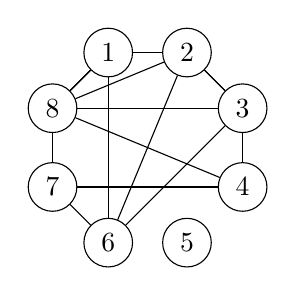
\begin{tikzpicture}[node distance=1cm]
\tikzstyle{vertex}=[draw,circle]
\node [vertex] (a){1};
\node [vertex,right of=a] (b){2};
\node [vertex,below right of=b] (c){3};
\node [vertex,below of=c] (d){4};
\node [vertex,below left of=d] (e){5};
\node [vertex,left of=e] (f){6};
\node [vertex,above left of=f] (g){7};
\node [vertex,above of=g] (h){8};
\path[every node/.style={font=\sffamily\small}]
    (a) edge node [above] {} (b)
    (a) edge node [left] {} (h);
\path[every node/.style={font=\sffamily\small}]
    (b) edge node [above] {} (a)
    (b) edge node [below] {} (c);
\path[every node/.style={font=\sffamily\small}]
    (c) edge node [below] {} (b)
    (c) edge node [left] {} (d)
    (c) edge node [left] {} (f);
\path[every node/.style={font=\sffamily\small}]
    (d) edge node [left] {} (g)
    (d) edge node [left] {} (h);
\path[every node/.style={font=\sffamily\small}]
    (f) edge node [above] {} (a)
    (f) edge node [below] {} (b);
\path[every node/.style={font=\sffamily\small}]
    (g) edge node [left] {} (d)
    (g) edge node [left] {} (f)
    (g) edge node [left] {} (h);
\path[every node/.style={font=\sffamily\small}]
    (h) edge node [above] {} (a)
    (h) edge node [below] {} (b)
    (h) edge node [left] {} (c);
\end{tikzpicture}
\end{center}

\paragraph{Matice souslednosti} reprezentuje graf o $n$ vrcholech pomocí matice $n\times n$, kde v $i$-tém sloupci a $j$-tém řádku je jednička, pokud
je $i$-tý vrchol s $j$-tým vrcholem spojený hranou, v opačném případě je tam nula. Výše uvedenému grafu by odpovídala matice (+ zápis v pythonu)
\begin{center}
\lstset{
numbers=none,
stepnumber=1,
numbersep=5pt,
numberstyle=\small\color{black}
}
\begin{minipage}{3.5cm}
$$
\left(
\begin{array}{cccccccc}
0 & 1 & 0 & 0 & 0 & 1 & 0 & 1\cr
1 & 0 & 1 & 0 & 0 & 1 & 0 & 1\cr
0 & 1 & 0 & 1 & 0 & 1 & 0 & 1\cr
0 & 0 & 1 & 0 & 0 & 0 & 1 & 1\cr
0 & 0 & 0 & 0 & 0 & 0 & 0 & 0\cr
1 & 1 & 1 & 0 & 0 & 0 & 1 & 0\cr
0 & 0 & 0 & 1 & 0 & 1 & 0 & 1\cr
1 & 1 & 1 & 1 & 0 & 0 & 1 & 0\cr
\end{array}
\right)
$$
\end{minipage}
\hskip2cm
\begin{minipage}{7cm}
\begin{python}
>>> g = [[0, 1, 0, 0, 0, 1, 0, 1],
	 [1, 0, 1, 0, 0, 1, 0, 1],
	 [0, 1, 0, 1, 0, 1, 0, 1],
	 [0, 0, 1, 0, 0, 0, 1, 1],
	 [0, 0, 0, 0, 0, 0, 0, 0],
	 [1, 1, 1, 0, 0, 0, 1, 0],
	 [0, 0, 0, 1, 0, 1, 0, 1],
	 [1, 1, 1, 1, 0, 0, 1, 0]]
\end{python}
\end{minipage}
\end{center}

\paragraph{Incidenční Matice.} Pokud má graf hodně vrcholů ale jen málo hran, může být výhodnější graf reprezentovat jako matici $n\times m$ ($m$ je počet hran), kde řádky
odpovídají hranám a sloupce vrcholům. V $i$-tém řádku jsou jedničky těch dvou sloupcích, které odpovídají vrcholům jež $i$-tá hrana spojuje. V ostatních sloupcích jsou nuly.
Výše uvedenému grafu by odpovídala matice (+ zápis v pythonu)
\begin{center}
\lstset{
numbers=none,
stepnumber=1,
numbersep=5pt,
numberstyle=\small\color{black}
}
\begin{minipage}{3.5cm}
$$
\left(
\begin{array}{cccccccc}
1 & 1 & 0 & 0 & 0 & 0 & 0 & 0\cr
1 & 0 & 0 & 0 & 0 & 0 & 0 & 1\cr
0 & 1 & 1 & 0 & 0 & 0 & 0 & 0\cr
0 & 1 & 0 & 0 & 0 & 1 & 0 & 0\cr
0 & 1 & 0 & 0 & 0 & 0 & 0 & 1\cr
0 & 0 & 1 & 1 & 0 & 0 & 0 & 0\cr
0 & 0 & 1 & 0 & 0 & 1 & 0 & 0\cr
0 & 0 & 1 & 0 & 0 & 0 & 0 & 1\cr
0 & 0 & 0 & 1 & 0 & 0 & 1 & 0\cr
0 & 0 & 0 & 1 & 0 & 0 & 0 & 1\cr
0 & 0 & 0 & 0 & 0 & 1 & 1 & 0\cr
0 & 0 & 0 & 0 & 0 & 0 & 1 & 1\cr
\end{array}
\right)
$$
\end{minipage}
\hskip2cm
\begin{minipage}{7cm}
\begin{python}
>>> g = [[1, 1, 0, 0, 0, 0, 0, 0],
	 [1, 0, 0, 0, 0, 1, 0, 0],
	 [1, 0, 0, 0, 0, 0, 0, 1],
	 [0, 1, 1, 0, 0, 0, 0, 0],
	 [0, 1, 0, 0, 0, 1, 0, 0],
	 [0, 1, 0, 0, 0, 0, 0, 1],
	 [0, 0, 1, 1, 0, 0, 0, 0],
	 [0, 0, 1, 0, 0, 1, 0, 0],
	 [0, 0, 1, 0, 0, 0, 0, 1],
	 [0, 0, 0, 1, 0, 0, 1, 0],
	 [0, 0, 0, 1, 0, 0, 0, 1],
	 [0, 0, 0, 0, 0, 1, 1, 0],
	 [0, 0, 0, 0, 0, 0, 1, 1]]
\end{python}
\end{minipage}
\end{center}

\paragraph{Seznam sousedů.} Při této reprezentaci si ke každému vrcholu pamatujeme seznam jeho ``sousedů'', t.j. vrcholů do nichž z něj vede hrana.
Výše uvedený graf by v pythonu byl reprezentován například takto:

{
\lstset{
numbers=none,
stepnumber=1,
numbersep=5pt,
numberstyle=\small\color{black}
}
\begin{python}
 >>> g = [[2, 6, 8],
	  [1, 3, 6, 8],
	  [2, 4, 6, 8],
	  [3, 7, 8],
	  [],
	  [1, 2, 3, 7],
	  [4, 6, 8],
	  [1, 2, 3, 4, 7]]
\end{python}
}

\begin{cviceni} Napište Pythonovské funkce pro převod grafu z jedné reprezentace do jiné.
\end{cviceni}

\subsection*{Komponenty souvislosti}

První grafový algoritmus, který si ukážeme, je algoritmus, který hledá tzv. komponenty
souvislosti. Uvažujme následující graf, který se rozpadá na tři části A, B, C (jak je naznačeno přerušovanou čarou).

\begin{center}
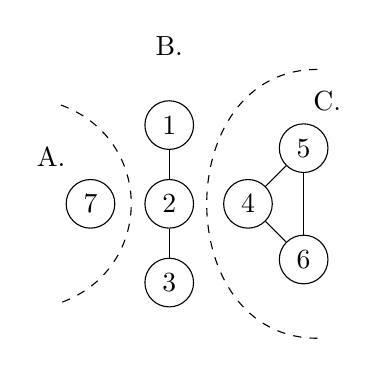
\begin{tikzpicture}[node distance=1cm]
\tikzstyle{vertex}=[draw,circle]

\node [vertex] (a){1};
\node [vertex,below of=a] (b){2};
\node [vertex,below of=b] (c){3};

\node [vertex,right of=b] (d){4};
\node [vertex,above right of=d] (e){5};
\node [vertex,below right of=d] (f){6};

\node [vertex,left of=b] (g){7};

\path[every node/.style={font=\sffamily\small}]
    (a) edge node [above] {} (b)
    (b) edge node [below] {} (c);

    \path[every node/.style={font=\sffamily\small}]
    (d) edge node [above] {} (e)
    (e) edge node [below] {} (f)
    (f) edge node [left] {} (d);

\node [below of=g,shift={(-5mm,-3mm)}] (gb) {};
\node [above of=g,shift={(-5mm,+3mm)}] (gu) {};
\node [below of=gu,shift={(0mm,+3mm)}] (kA) {A.};

\node [below of=f,shift={(3mm,-0mm)}] (bf) {};
\node [above of=e,shift={(3mm,+0mm)}] (ue) {};
\node [below of=ue,shift={(0mm,+6mm)}] (kC) {C.};

\node [above of=a,shift={(0mm,+0mm)}] (kB) {B.};
    
\draw[dashed,-]
    (gu) .. controls +(-20:14mm) and +(20:14mm) .. (gb);
    
\draw[dashed,-]
    (ue) .. controls +(180:20mm) and +(-180:20mm) .. (bf);

\end{tikzpicture}
\end{center}

Těmto částem se říká tzv. komponenty souvislosti. Mají tu vlastnost, že mezi
jednotlivými částmi nevede žádná hrana a naopak v jednotlivých částech se
lze z libovolného uzlu po hranách dostat do libovolného jiného. To je obsahem
následující definice.

\begin{definition} Posloupnost vrcholů $v_1,\ldots,v_k$ grafu $(V,E)$ nazveme \emph{cestou}, pokud pro $i=1,\ldots,k-1$
platí, že $v_iEv_{i+1}$. Graf $(V,E)$ je souvislý, pokud z každého vrcholu vede cesta do každého jiného vrcholu, t.j. 
pokud pro všechna $v\neq w\in V$ existuje cesta $v_1,\ldots, v_k$ taková, že $v=v_1$ a $w=v_k$. Komponentou
souvislosti rozumíme nějakou maximální souvislou podmnožinu $K\subseteq V$, t.j. takovou podmnožinu, že mezi každými
dvěma prvky $K$ existuje cesta a přidáním jakéhokoliv dalšího prvku do $K$ toto přestane platit.
\end{definition}

Ukážeme si algoritmus, který k danému vrcholu nalezne komponentu souvislosti, do které vrchol patří (uvědomte si, že každý vrchol patří do nějaké komponenty souvislosti).
Algoritmus funguje tak, že začne v zadaném vrcholu a postupně prochází všechny jeho
sousedy a sousedy jeho sousedů atd., dokud to lze. V okamžiku, kdy už nemůže dál,
našel komponentu souvislosti. Kód v pythonu je uveden ve výpisu \ref{alg:komponentysouvislosti}.

\src{komponentysouvislosti}{Komponenta Souvislosti}

\begin{todo}
Procházení do hloubky vs. procházení do šířky
\end{todo}


\subsection*{Obarvení grafu}

Nyní si popíšeme jednoduchý algoritmus, který nalezne relativně dobré obarvení grafu. Algoritmus patří do třídy ``hladových''
algoritmů. Hladové se jim říká proto, že v každém kroku provedou akci, která se nabízí jako první --- t.j. nemyslí dopředu.
V našem případě bude algoritmus procházet vrcholy v nějakém pořadí a v každém kroku přiřadí vrcholu, který je právě na řadě,
nejmenší barvu, kterou může --- t.j. nejmenší takovou, která ještě nebyla přirazena žádnému jeho sousedu. Problém tohoto algoritmu
je v tom, že v závislosti na pořadí, ve kterém vrcholy prochází, může nalézt obarvení velmi špatné. Uvažujme například 
následující (\emph{bipartitní}) graf a jeho dvě možná obarvení vzniklá hladovým algoritmem (řady čísel nad obarvenými grafy udávají, 
v jakém pořadí algoritmus vrcholy procházel):

\begin{center}
\begin{minipage}{4cm}
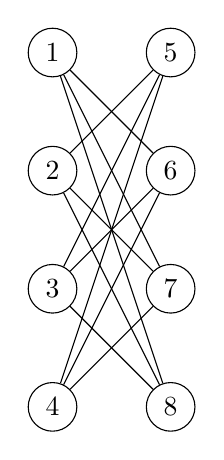
\begin{tikzpicture}[node distance=1.5cm]
\tikzstyle{vertex}=[draw,circle]
\node [vertex] (a){1};
\node [vertex,below of=a] (b){2};
\node [vertex,below of=b] (c){3};
\node [vertex,below of=c] (d){4};

\node [vertex,right of=a] (e){5};
\node [vertex,below of=e] (f){6};
\node [vertex,below of=f] (g){7};
\node [vertex,below of=g] (h){8};
\path[every node/.style={font=\sffamily\small}]
(a) edge node {} (f)
(a) edge node {} (g)
(a) edge node {} (h)
(b) edge node {} (e)
(b) edge node {} (g)
(b) edge node {} (h)
(c) edge node {} (e)
(c) edge node {} (f)
(c) edge node {} (h)
(d) edge node {} (e)
(d) edge node {} (f)
(d) edge node {} (g);
\end{tikzpicture}
\end{minipage}
\begin{minipage}{4cm}
\begin{center}
1, 2, 3, 4, 5, 6, 7, 8.
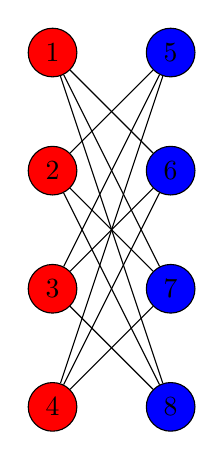
\begin{tikzpicture}[node distance=1.5cm]
\tikzstyle{vr}=[draw,circle,fill=red]
\tikzstyle{vb}=[draw,circle,fill=blue]
\node [vr] (a){1};
\node [vr,below of=a] (b){2};
\node [vr,below of=b] (c){3};
\node [vr,below of=c] (d){4};

\node [vb,right of=a] (e){5};
\node [vb,below of=e] (f){6};
\node [vb,below of=f] (g){7};
\node [vb,below of=g] (h){8};
\path[every node/.style={font=\sffamily\small}]
(a) edge node {} (f)
(a) edge node {} (g)
(a) edge node {} (h)
(b) edge node {} (e)
(b) edge node {} (g)
(b) edge node {} (h)
(c) edge node {} (e)
(c) edge node {} (f)
(c) edge node {} (h)
(d) edge node {} (e)
(d) edge node {} (f)
(d) edge node {} (g);
\end{tikzpicture}
\end{center}
\end{minipage}
\begin{minipage}{4cm}
\begin{center}
1,5,2,6,3,7,4,8
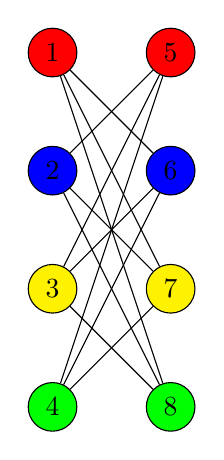
\begin{tikzpicture}[node distance=1.5cm]
\tikzstyle{va}=[draw,circle,fill=red]
\tikzstyle{vb}=[draw,circle,fill=blue]
\tikzstyle{vc}=[draw,circle,fill=yellow]
\tikzstyle{vd}=[draw,circle,fill=green]
\node [va] (a){1};
\node [vb,below of=a] (b){2};
\node [vc,below of=b] (c){3};
\node [vd,below of=c] (d){4};

\node [va,right of=a] (e){5};
\node [vb,below of=e] (f){6};
\node [vc,below of=f] (g){7};
\node [vd,below of=g] (h){8};
\path[every node/.style={font=\sffamily\small}]
(a) edge node {} (f)
(a) edge node {} (g)
(a) edge node {} (h)
(b) edge node {} (e)
(b) edge node {} (g)
(b) edge node {} (h)
(c) edge node {} (e)
(c) edge node {} (f)
(c) edge node {} (h)
(d) edge node {} (e)
(d) edge node {} (f)
(d) edge node {} (g);
\end{tikzpicture}
\end{center}
\end{minipage}
\end{center}

Je tedy velmi důležité vhodně zvolit pořadí, ve kterém se vrcholy procházejí. Protože je problém NP-těžký, nemůžeme čekat, že
se nám podaří vždy zvolit optimální pořadí. Nicméně existují různé heuristiky, z nichž si jednu ukážeme (viz \cite{Brelaz:1979}). 
Nejdříve potřebujeme definici:

\begin{definition} Saturovaností vrcholu $v$ (značíme $sat(v)$) budeme rozumět počet různých barev, které jsou přiřazeny
sousedícím vrcholům.
\end{definition}

Pořadí budeme volit následovně. Vrcholy si uspořádáme sestupně podle jejich stupně (t.j. podle počtu sousedů). V každém kroku
zvolíme ze zbývajících vrcholů ten vrchol, který má největší saturovanost. Pokud je takových vrcholů více, zvolíme vrchol 
největšího stupně. Zkusme nyní tento algoritmus zapsat v pythonu. Graf budeme reprezentovat jako pythonovský {\tt dict}, který bude
indexován vrcholy a bude obsahovat pro každý vrchol seznam jeho sousedů. Zároveň bude ke každému vrcholu ještě obsahovat
seznam barev přiřazených jeho sousedům (pro výpočet saturovanosti).


\begin{center}
\begin{minipage}{7cm}
\srchere{colorgraph}{Heuristické barvení grafu}
\end{minipage}
\begin{minipage}{4cm}
\begin{center}
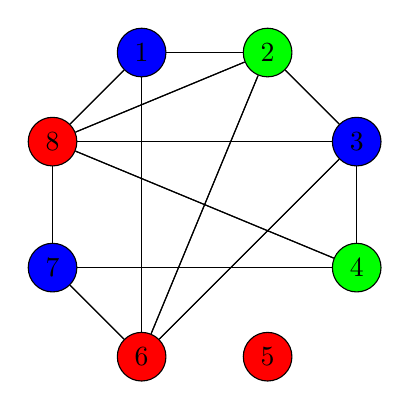
\begin{tikzpicture}[node distance=1.6cm]
\tikzstyle{vertexB}=[draw,circle,fill=blue]
\tikzstyle{vertexC}=[draw,circle,fill=green]
\tikzstyle{vertexB}=[draw,circle,fill=blue]
\tikzstyle{vertexC}=[draw,circle,fill=green]
\tikzstyle{vertexA}=[draw,circle,fill=red]
\tikzstyle{vertexA}=[draw,circle,fill=red]
\tikzstyle{vertexB}=[draw,circle,fill=blue]
\tikzstyle{vertexA}=[draw,circle,fill=red]

\node [vertexB] (B){1};
\node [vertexC,right of=B] (C){2};
\node [vertexB,below right of=C] (D){3};
\node [vertexC,below of=D] (E){4};
\node [vertexA,below left of=E] (F){5};
\node [vertexA,left of=F] (G){6};
\node [vertexB,above left of=G] (H){7};
\node [vertexA,above of=H] (I){8};

\path[every node/.style={font=\sffamily\small}]
 (B) edge node {} (C) 
 (B) edge node {} (G) 
 (B) edge node {} (I) 
 (C) edge node {} (B) 
 (C) edge node {} (D) 
 (C) edge node {} (G) 
 (C) edge node {} (I) 
 (D) edge node {} (C) 
 (D) edge node {} (E) 
 (D) edge node {} (I) 
 (D) edge node {} (G) 
 (E) edge node {} (D) 
 (E) edge node {} (I) 
 (E) edge node {} (H) 
 (G) edge node {} (D) 
 (G) edge node {} (C) 
 (G) edge node {} (B) 
 (G) edge node {} (H) 
 (H) edge node {} (G) 
 (H) edge node {} (E) 
 (H) edge node {} (I) 
 (I) edge node {} (H) 
 (I) edge node {} (E) 
 (I) edge node {} (D) 
 (I) edge node {} (C) 
 (I) edge node {} (B);
\end{tikzpicture}
\end{center}
\end{minipage}
\end{center}


\subsection*{Hledání cesty v grafu (Dijkstrův algoritmus)}

Pojďme se podívat ještě na jednu typickou úlohu, která má navíc praktické využití. Půjde o hledání nejkratší cesty v grafu. Jako motivace nám může posloužit příklad
grafu ze začátku kapitoly. Tam jsme si ukazovali graf silniční sítě, ve kterém vrcholy odpovídaly jednotlivým městům a hrany silnicím. V této situaci bychom mohli chtít
zjistit, jaká je nejkratší cesta z Prahy do Brna. K tomu budeme potřebovat nejen
původní graf, ale i informace o délkách jednotlivých hran. Naší úlohu můžeme nyní
formulovat v řeči grafů třeba následovně:

\begin{question} Mějme dán graf $G=(V,E)$, spolu s funkcí $d:E\to\mathbb{R}$ (udávající
délky hran) a dva vrcholy $a,b\in V$. Nalezněte cestu $a_0,\ldots,a_n$ z $a$ do $b$ (t.j. $a_0=a, a_n=b$) takovou, aby hodnota
\begin{displaymath}
 \sum_{i=0}^{n-1} d(a_i,a_{i+1})
\end{displaymath}
byla co nejmenší.
\end{question}

Ukážeme si algoritmus, který vymyslel nizozemský informatik \person{Dijkstra} (viz \cite{Dijkstra:59}). 

Algoritmus je založen na následující myšlence. Pokud bychom postupně procházeli všechny možné cesty začínající v počátečním vrcholu 
$a$ do nějakého jiného vrcholu v pořadí od nejkratších k nejdelším, pak bychom ve chvíli, kdy poprvé narazíme na cestu, která končí ve vrcholu $b$, 
byli hotovi. Tato cesta by totiž musela být nejkratší --- všechny pozdější cesty jsou delší, všechny dřívější skončily v jiném vrcholu.

Algoritmus tedy začne v počátečním vrcholu a postupně prochází v určitém pořadí 
vrcholy grafu. V průběhu svého výpočtu si pro každý vrchol pamatuje dvě informace. 
První informací je délka nejlepší cesty z počátečního vrcholu do tohoto vrcholu, 
kterou zatím našel. Druhou informací je sousední vrchol, ze kterého sem tato nejkratší cesta vedla. 

Zbývá určit, v jakém pořadí prochází vrcholy. V každém kroku si z dosud nenavštívených vrcholů
vybere ten vrchol, do kterého vede nejkratší cesta. Do něj se přemístí a upraví informace
o nejkratší cestě u všech jeho sousedů. Implementace v Pythonu může vypadat například
tak, jako na výpisu \ref{alg:dijkstra}.

\varsrc[lastline=69]{dijkstra}{Dijkstrův algoritmus}

Jaká je složitost tohoto algoritmu? Algoritmus navštíví každý vrchol nejvýše jednou,
tedy while cyklus (řádky 35--57) se provede nejvýše $|V|$, kde $|V|$ je počet vrcholů.
V každé iteraci se musí projít všichni sousedé aktuálního vrcholu (řádky 37--42),
těch může být nejvýše $|V|$, pak se musí vybrat vrchol s nejkratší cestou (řádek 46),
což v naší implementaci znamená opět $|V|$ kroků. Nakonec se rekonstruuje cesta (řádek
57, volání funkce {\tt postav\_cestu}), to se však děje pouze jednou za celý běh a
na složitost to nemá vliv. Celkem tedy dostáváme $O(|V|(|V|+|V|)) = O(|V|^2)$. 

Za předpokladu, že většina vrcholů má jen málo sousedů, se dá algoritmus vylepšit.
Pokud bychom si průběžné informace o nejlepších cestách neukládali jako seznam
ale jako haldu, dostali bychom odhad $O((|E|+|V|)\log|V|)$. Ještě lepšího výsledku
$O(|E| + |V|\log|V|)$ bychom dosáhli nahrazením haldy její variantou nazývanou \emph{\href{http://en.wikipedia.org/wiki/Fibonacci_heap}{Fibonnaciho halda}} (viz \cite{Tarjan:1984}).



\ifx\ucebnice\undefined
\renewcommand{\refname}{\textbf{Literatura}}
\bibliographystyle{mujstyl}
\bibliography{ref}

\end{document}
\fi